\documentclass{article}

\usepackage{arxiv}

\usepackage{amsmath, amssymb}
\usepackage{cite}
\usepackage{graphicx}
\graphicspath{ {./images/} }
\usepackage{placeins}
\usepackage[utf8]{inputenc} % allow utf-8 input
\usepackage[T1]{fontenc}    % use 8-bit T1 fonts
\usepackage{hyperref}       % hyperlinks
\usepackage{url}            % simple URL typesetting
\usepackage{booktabs}       % professional-quality tables
\usepackage{amsfonts}       % blackboard math symbols
\usepackage{nicefrac}       % compact symbols for 1/2, etc.
\usepackage{microtype}      % microtypography
\usepackage{cleveref}       % smart cross-referencing
\usepackage{lipsum}         % Can be removed after putting your text content
\usepackage{graphicx}
%\usepackage{natbib}
\usepackage{doi}


\title{Cash Flow Dispersion Model,  An Application of the \emph{Economic Order Quantity} to Personal Finance}

% Here you can change the date presented in the paper title
%\date{September 9, 1985}
% Or remove it
%\date{}

\newif\ifuniqueAffiliation
% Uncomment to use multiple affiliations variant of author block 
\uniqueAffiliationtrue

\ifuniqueAffiliation % Standard variant of author block
\author{\hspace{1mm}Anthony B. Trevi\~{n}o\\
	Computer Science Graduate Student, Cloud Technologist\\
	Georgia Institute of Technology, Ant Finance LLC\\
	\text{trevino293@gmail.com} \\
	%% examples of more authors
	%% \AND
	%% Coauthor \\
	%% Affiliation \\
	%% Address \\
	%% \texttt{email} \\
	%% \And
	%% Coauthor \\
	%% Affiliation \\
	%% Address \\
	%% \texttt{email} \\
	%% \And
	%% Coauthor \\
	%% Affiliation \\
	%% Address \\
	%% \texttt{email} \\
}

% Uncomment to override  the `A preprint' in the header
%\renewcommand{\headeright}{Technical Report}
%\renewcommand{\undertitle}{Technical Report}
\renewcommand{\shorttitle}{\textit{Cash Flow Dispersion Model}}

%%% Add PDF metadata to help others organize their library
%%% Once the PDF is generated, you can check the metadata with
%%% $ pdfinfo template.pdf
\hypersetup{
pdftitle={Cashflow Dispersion Model},
pdfsubject={q-bio.NC, q-bio.QM},
pdfauthor= {Anthony Trevino},
pdfkeywords={Economic Order Quantity, Personal Finance, Asset Management, Inventory Management}
}

\begin{document}
\maketitle

\begin{abstract}

This paper defines a cash flow dispersion model that minimizes liquid assets inventory whilist comfortably maintaining the ability to meet periodic demand. Migrating excess liquid asset inventory gained to long term asset inventory, thus increasing the amount of assets available to gain interest. Cumulative average estimates are used to account for variation in investment returns and cash flow habits. The resulting aggregate estimates of cash flows, liquid assets, long term assets and long term assets return percentage will be used to determine economic reorder point and order quantity. Dollars which can be considered equal to inventory will be migrated between long term and liquid asset balances based upon the economic order quantity and an intuitive investment threshold. This model can be used to understand a target cash flow state, providing target account values, triggers, order quantity kickstarting progression toward confident cash flow forecasting for an individual or corporation. With the expansion of deep learning algorithms and open banking, the ability to predict and measure performance against this model may be attainable in future study. 

\textbf{Github: \url{https://github.com/trevino293/CFD/tree/main}}

\end{abstract}


% keywords can be removed
\keywords{Economic Order Quantity \and Personal Finance \and Asset Management \and Inventory Management \and Cash Flow Dispersion Model}

\section{Preface}
This is my first draft and attempts to apply engineering theory and mathematics to solve a complex problem. The problem statement is defined as running out of funds in the final stages of life due to poor planning and optimization of assets. I once read a statistic stating that the median of Americans aggregate savings is \$570 and on average \$33,000. Whether these numbers are accurate or not is beside the problem, the range that they are in is not near an acceptable level for long term feasibility.

It is important to understand that this is my first attempt at creating a mathematically valid and acceptable model. Without in depth graduate level or higher qualifications in these subjects my attempt at the model is just that, an attempt. I understand that there will be critique and learning opportunities through development and feedback of this model, I welcome this. I have created this for fun and really couldn't get my mind away from the problem as I embark on my own personal asset management journey. Therefore I tried to write it up for more clarity, reference and validation. I hope to help others by applying this model, automated through a website, generating long term asset estimates and other financial metrics that could provide insight to potential asset positions over time.

\textbf{Model Development Timeline:}\\
$\bullet$ \; Initial idea and documentation in April 2019.\\
$\bullet$ \; Refinement for arxiv.org and peer review in December 2023. \\

\section{Introduction}

The objective is to minimize liquid assets inventory whilst comfortably maintaining ability to meet periodic demand. Additionally migrating excess liquid asset inventory gained to long term asset inventory, thus increasing the amount of assets available to gain interest. Significantly increasing  the amount of savings available to gain interest through application of the economic order quantity model to aggregate liquid assets. First define an aggregate estimate of period based cash flows generating net change per period. The net change is applied to the liquid asset balance following the inventory demand distribution. This demand distribution will be used to compute the economic order quantity $Q_{i}$ to order and reorder point $r_{i}$ per period. 

Relating $Q_{i}$ and $r_{i}$ to personal asset management, liquid asset balance will be defined as inventory $I_{i}$. Liquid assets encompass cash assets or any money that is used frequently and can be readily accessed, usually will not gain interest.  A 0\% return on investment account is influencing the liquid asset balance per period, an $i$ period will be on the same interval as the sample net change of cash flows. The objective is to minimize inventory, migrating as much assets to long term assets balance $S_{i}$, your future self in the account that will be gaining interest. Long term assets also will have to aggregated to a single amount but in addition tied to an investment return rate $i$. This will be used to model the increase of long term asset balance over time.\\

I notice large places for variation within the model, expecting someone to provide accurate forecast inclusive of all credits and debits per period is unlikely. Similarly trying to estimate an accurate aggregate investment return percentage with many distributed investment assets. However I believe by asking about the confidence in the ability to adhere to the estimates provided, a confidence interval of demand can be applied to model some of this variation.  

\begin{figure}
	\centering
	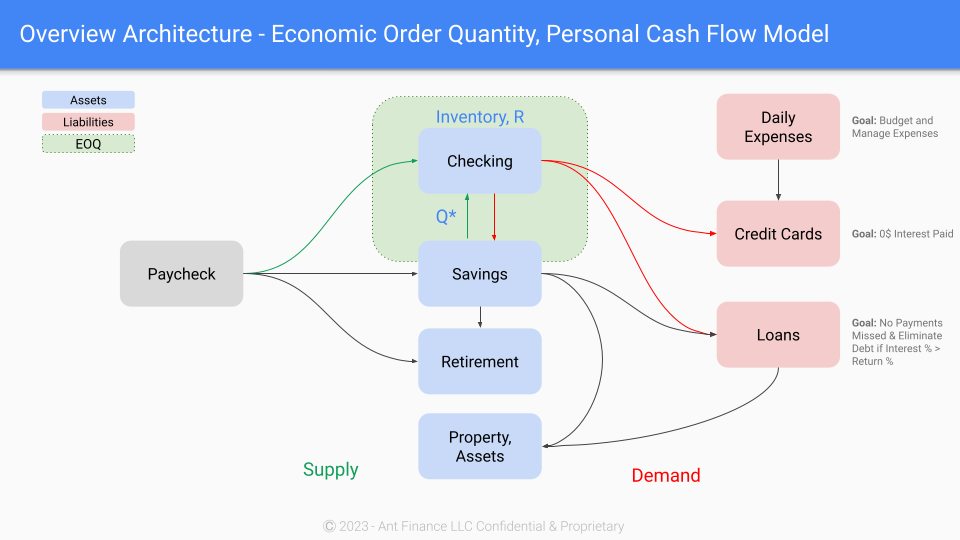
\includegraphics[width=11cm, height=7cm]{EOQ Personal Cash Flow Model}
	\caption{Overview Architecture}
	\label{fig:fig1}
\end{figure}
\FloatBarrier

\section{Methodology}
Adapt and apply the economic order quantity model shown in professor Ronald Askin’s IEE 461 \cite{Askin2019} production control course to generate a feasible mathematical model which minimizes aggregate liquid asset balance and maximize long term assest exposure to gains. 

\subsection{Demand and Net Change}
Aggregate liquid asset balance per period  $I_{i}$ will be estimated through sampling the net change to a theoretical ‘master checking account’ which can account for all cash flow within the period. Cash will be dispersed through spending, holding and investing money. Dispersion provides the net change per period $NC_{i}$, translating to a demand distribution shown below.

\begin{equation}
	\begin{split}
		if \; NC_{i} < 0 \;\implies D_{i} = |NC_{i}| \\
	  	\:\text{else}\; D_{i} = 0
	\end{split}
\end{equation}
 
\subsection{Investment Criterion}
This distribution is based upon that when cumulative net change within a period is greater than 0 money was gained, therefore there is no impact or demand on the liquid asset balance, only surplus cash. This surplus will be addressed through investing at the end of the period if liquid asset balance surpases the reorder point plus order quantity plus investment amount or $Y_{i}$ the Investment threshold. A defined target investment quantity $z$ will be used to calculate the investment threshold. 

The investment threshold value  $Y_{i} =  r_{i} + Q_{i} + z$  is a first instinct to me as when I would feel comfortable to invest. My inventory or liquid assets would have more than the entire amount to be invested plus one economic order quantity plus the economic reorder point. A substantial buffer of inventory left after the investment is removed. Additionally the actual amount invested will be the current inventory minus the investment threshold, minus demand or $I_{i} - Y_{i} - D_{i}$  I believe this will give strong resistance to changes in demand and allow the inventory to remain positive over time, reducing the exposure to negative assets, debt. 

\begin{equation}
	\begin{split}
		\text{Invest if} \: I_{i} > r_{i} + Q_{i} + z \:\text{and} \: I_{i} - ( I_{i} - r_{i} - Q_{i} - z) - D_{i} > 0 \\
		\text{Investment threshold} \: Y_{i} =  r_{i} + Q_{i} + z 
	\end{split}
\end{equation}

\subsection{Liquid Assets}
The economic order quantity or $Q_{i}$  asssets will be removed from long term assets to meet demand when the liquid assets inventory falls below the re-order point $r_{i}$.

\begin{align*}
	& if \; I_{i} > Y_{i} \;\implies\;	 \Delta_{i} = I_{i} - Y_{i} - D_{i}\\
	& if \; I_{i} < 0 \;\implies\; 	 \Delta_{i} = I_{i}\\ 
	\\
	& \text{Net Change} \: = NC_{i}= Q_{i-1} - \Delta_{i-1}\\
										\implies & I_{i} = I_{i-1} + NC_{i}\\
\end{align*}

\subsection{Long Term Assets}
Aggregate long term assets per period $S_{i}$ is an estimated value of all long term saving methods. Aggregate investment return $i$ is an estimated average return percentage of all long term saving methods.  This balance will be gaining investments $\Delta_{i}$, interest at $i$ and losing economic order quantities $Q_{i}$. The resulting long term assets distribusion is defined by the following. 

\begin{align*}
	if \; I_{i} > Y_{i} \; \text{and} \: I_{i} - \Delta_{i|+} - D_{i} > 0 	& \implies \;\;\; S_{i} = S_{i-1}(1+i_{i-1}) + ( \Delta_{i-1})\\
	if \; 0 < I_{i} < r_{i} 							& \implies \;\;\; S_{i} = S_{i-1}(1+i_{i-1}) - Q_{i-1}\\
	if \; I_{i} < 0  								& \implies \;\;\; S_{i} = S_{i-1}(1+i_{i-1}) - Q_{i-1} +  \Delta_{i-1}\\
\end{align*}

\section{Example Problem}
The following section will be an example and explanation of each parameter within the economic order quantity model relating to this application. These are an adaptation of the parameters defined to build the economic order quantity model which were shown in the course \cite{Askin2019} being applied to inventory management, rather than asset flow.

\subsection{Variable Definiton}  

These formulas were presented during lecture \cite{Askin2019} in the context of warehouse inventory mangement, I attempt to adapt and transform these values for this context. 

\begin{description}
	\item[Holding Costs:] $= h_{i}$ = \; $ i \:C\: \overline{I} $
	\item[Return:] $ i $ = estimate return on long term assets
	\item[Cost per Unit:] C = $1\$ =1 \; Unit $
	\item[Average Inventory, Liquid Assets:] $\overline{I} \; \implies \; \overline{I}_{i} = \frac{1}{i}\sum_{i=0}^{i}I_{i}$
	\item[Setup Cost:]  = $\frac{AD}{Q}$
	\item[Income:]  = $A_{i}$ = Approximate cash generated per period
	\item[Net Change:]= $NC_{i}$ = \; Sum of all Cash flows in period \; $=CF_{i}^{+}-CF_{i}^{-}$
	\item[Demand:]= $\overline{D}_{i} = \frac{1}{i + 1}\sum_{i=0}^{i-1}|NC_{i}| \implies \; \frac{1}{i + 1}\sum_{i=0}^{i-1}D_{i}$
	\item[Economic Order Quantity:]= $Q_{i}$
	\subitem[if $I_{i} < r_{i}$] $\implies\;  Q_{i} = \sqrt{\frac{2A_{i}\overline{D_{i}}}{h_{i}}}$
	\subitem[if $I_{i} > r_{i}$]$ \implies\;  Q_{i} = 0$
	\item[Re-Order Point:]= $r_{i} = \tau_{A} \overline{D_{i}}$
	\item[Lead Time :]= $\tau_{A}$ = Lead time between paychecks or aggregate income flow and transfer time
\end{description}

\subsection{Example Problem}

\begin{flushleft}
\textbf{Google Sheets Example Problem}
 \url{https://docs.google.com/spreadsheets/d/19UFwlwobvhcvf8LA1VnPy0XWBtuGiWFGkX-fbACpsl4/edit?usp=sharing}
\end{flushleft}

The following is a sample of questions and data points to initiate the model. 

\begin{description}
	\item[$\bullet$ Long Term Asset Return:] $5\% \: \implies i = 5\%$
	\item[$\bullet$ Personal Statement on Cash/Balance:] "Maintain 4000\$ in checking and 200 cash"
	\item[$\bullet$ Personal Statement on Spend/Demand:] "Spend roughly 500 dollars a week in daily expenses and have 1200 in monthly costs"
	\item[$\bullet$ Personal Statement on Income:] "I make 1000 dollars weekly after tax" $\: \implies$ Weekly $A_{i} =  1000 $
	\item[$\bullet$ Personal Statement on Savings:] "I have 98,000 dollars saved and plan to save 30\% of all paychecks" $\: \implies$ \: $S_{0} =  98000 $
	\subitem[$\implies \: z =  1000*.3 = 300 $]
	\item[$\bullet$ Personal Statement on Expected Demand:] "I have 2000 dollar loan that I will pay off in 2 weeks" $\: \implies$ \: $D_{2} =  D_{2} + 2000 $
\end{description}

\subsubsection{Step 1 - Initiate}

\begin{equation}
	\begin{split}
		I_{0} = 1000 - 1200 -500 + 4200 = 3500\\
		NC_{0} = 1000 - 1200 - 500 = -700\\
		weekly h_{0} = (.05/52 weeks)(\$1)(\$3500) = h_{0} = 3.4 \\
		\implies \overline{I_{0}} =  3500 \\
		\implies D_{0} = |NC_{0}|  = 700 \\
		\implies \overline{D_{0}} = 700 
	\end{split}
\end{equation}
\FloatBarrier

\begin{equation}
	\begin{split}
		Q_{0} =  \sqrt{\frac{2(1000)(700)}{3.4}} = 645\\
		I_{0} > r_{0} =3500 > 700 \implies Q_{0} = 0\\
		r_{0} =  \tau\overline{D_{i}} = \overline{D_{i}} = 700\\
		\implies \tau = \text{1 week of work time to generate paycheck}\\
		Y_{0} = Q_{0} + r_{0} + z = 645 + 300 + 700 = 1645\\
		\implies \: 3500 - 1645 - 700 > 0  = True \\
		\Delta_{0} = -1155
	\end{split}
\end{equation}
\FloatBarrier

\begin{table}
	\caption{$i = 0$ Initiate Model}
	\centering
	\begin{tabular}{||c|c|c|c|c|c|c|c|c|c|c||}
		\toprule
		$i$     & $NC_{i}$     & $D_{i}$ &  $\overline{D_{i}}$ & $I_{i}$ &  $\overline{I_{i}}$ & $I_{i}  - Y_{i} - D_{i} > 0$ & $\Delta_{i}$ & $S_{i}$ & $I_{i} < r_{i}$ & $(Q_{i}, r_{i})$\\
		\midrule
		0	& -700	&  700  	& 700  		& 3500	& 3500		& $1155 > 0$		 & -1155		& 98000 	&	No 	& (0, 700) \\
		\bottomrule
	\end{tabular}
	\label{tab:table}
\end{table}

\subsubsection{Step 2 - First Iteration and Action}

\begin{equation}
	\begin{split}
		I_{1} = 3500 - 700 = 2800\\
		NC_{1} = 1000 - 1155 - 500 = -655\\
		weekly h_{1} = (.05/52 weeks)(\$1)(\$3150) = h_{1} = 3.0\\
		\implies \overline{I_{1}} =  3150 \\
		\implies D_{1} = |NC_{1}|  = 655 \\
		\implies \overline{D_{1}} = (700+ 655)/2) = 677.5
	\end{split}
\end{equation}

\begin{equation}
	\begin{split}
		Q_{1} =  \sqrt{\frac{2(1000)(677.5)}{3.0}} = 668.9\\
		I_{1} > r_{1} = 2800 > 677.5 \implies Q_{1} = 0\\
		r_{1} =  \tau\overline{D_{1}} = \overline{D_{1}} = 677.5\\
		\implies \tau = \text{1 week of work time to generate paycheck}\\
		Y_{0} = Q_{0} + r_{0} + z = 668.9 + 300 + 677.5 = 1646.4\\
		\implies \: 2800 - 1646.4 - 655 > 0  = True \\
		\Delta_{0} = -498.6
	\end{split}
\end{equation}

\begin{equation}
	\begin{split}
		S_{1} =  S_{0}(1+(i/52)) - Q_{0} - \Delta_{0} \\
		S_{1} =  98000(1+(.05/52)) - 0 - (-1155) = 99249.25
	\end{split}
\end{equation}

\begin{table}
	\caption{$i = 1$ First Iteration}
	\centering
	\begin{tabular}{||c|c|c|c|c|c|c|c|c|c|c||}
		\toprule
		$i$     & $NC_{i}$     & $D_{i}$ &  $\overline{D_{i}}$ & $I_{i}$ &  $\overline{I_{i}}$ & $I_{i}  - Y_{i} - D_{i} > 0$ & $\Delta_{i}$ & $S_{i}$ & $I_{i} < r_{i}$ & $(Q_{i}, r_{i})$\\
		\midrule
		0	& -700	&  700  	& 700  		& 3500	& 3500		& $1155 > 0$		 & -1155		& 98000 	&	No 	& (0, 700) \\
		1	& -655	&  655 	& 677.5 		& 2800	& 3150		& $498.6 > 0$		 & -498.6		& 99249.25 	&	No 	& (0, 677.5) \\
		\bottomrule
	\end{tabular}
	\label{tab:table}
\end{table}

\begin{table}
	\caption{$i = 2,3$ Second and Third Iterations}
	\centering
	\begin{tabular}{||c|c|c|c|c|c|c|c|c|c|c||}
		\toprule
		$i$     & $NC_{i}$     & $D_{i}$ &  $\overline{D_{i}}$ & $I_{i}$ &  $\overline{I_{i}}$ & $I_{i}  - Y_{i} - D_{i} > 0$ & $\Delta_{i}$ & $S_{i}$ & $I_{i} < r_{i}$ & $(Q_{i}, r_{i})$\\
		\midrule
		0	& -700	&  700  	& 700  		& 3500	& 3500		& $1155 > 0$		 & -1155		& 98000 	&	No 	& (0, 700) \\
		1	& -655	&  655 	& 677.5 		& 2800	& 3150		& $498.6 > 0$		 & -498.6		& 99249.25 	&	No 	& (0, 677.5) \\
		2	& -1998.6	&  1998.6	& 1117.9 		& 2144.98	& 2815		& $-2180.32 > 0$		 &  0			& 99843.29 	&	No 	& (0, 1117.5) \\
		3	& 500		&  0		& 838.4		& 146.37	& 2147.8		& $-1893.5  > 0$		 &  0			& 99939.30 	&	Yes 	& (901.1, 838.4) \\
		\bottomrule
	\end{tabular}
	\label{tab:table}
\end{table}
\FloatBarrier


\begin{figure}
	\centering
	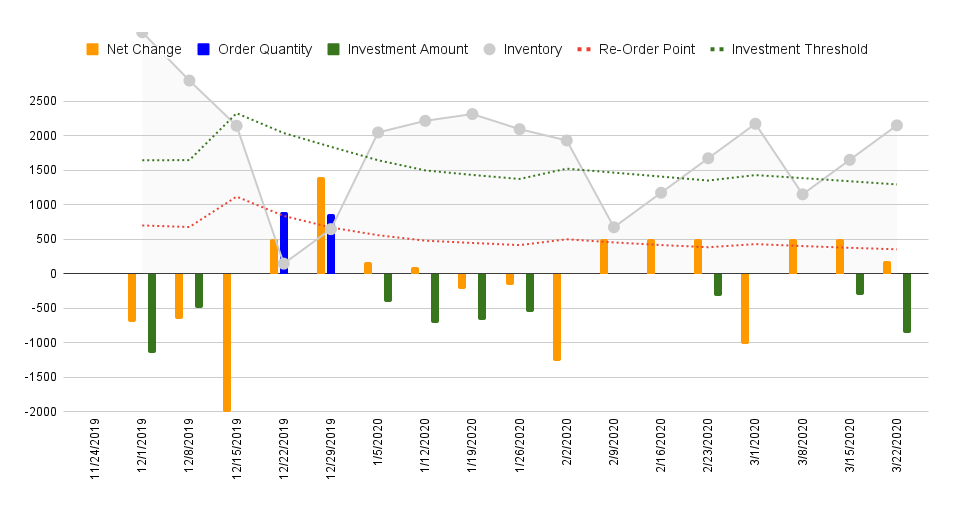
\includegraphics[width=17cm, height=10cm]{chart}
	\caption{Example chart with 2000 Loan in period 2}
	\label{fig:fig2}
\end{figure}
\FloatBarrier

In this example we can begin to see the models impact on long term and liquid assets balance. Initially the expected demand and current assets indicated a need to invest which was done in period  zero and one with 1155 and 498 dollar investments to long term assets. However a unusually high demand is required in period two, causing the balance to sink below the re-order point triggering two economic order quantity orders from the long term assets in periods three and four. When modeled for the remainder of the year with static demand and income no more orders are incurred. Indicating a positive net balance of demand and income, providing the ability to save in each period. Without proper understanding of budget and income this model may not be useful. 

\section{Conclusion}
I believe this model may be beneficial to society, helping others to understand and predict an accurate estimate of financial state optimized for exposure to gains. This is my first attempt at academic research and exploration I have composed these thoughts for more qualified expert peer review. I feel this work falls under the operations research domain as an extension of the Economic Order Quantity \cite{Askin2019}, but also believe future exploration may be in the economics, asset management and computer science domains. Application of this model in conjunction with the advancing technologies of deep learning as well as indutry trend toward open banking, with the right team and research I believe this model could be deployed and readily accesible. Providing mathematically backed investment and re-order points along with order quantity and investment amounts will be powerful. The challenge is in accurate prediciton of demand which will be reliant upon the model developer or user input untill all cash flows can be accounted for which will be impossible to predict. I will continue to explore this model with different payment periods, cashflow and random demand distribution based upon confidence in historic average demand.
Thank you for taking the time to review my work! 

\bibliographystyle{unsrtnat}
%%% \bibliography{references.bib}  %%% Uncomment this line and comment out the ``thebibliography'' section below to use the external .bib file (using bibtex) .

%%% Uncomment this section and comment out the \bibliography{references} line above to use inline references.
 \begin{thebibliography}{1}

 	\bibitem{Askin2019}
 	Ronald Askin (2019) \emph{Chapter 6, Inventory Management and the EOQ}, Lecture 5 IEE 461, Arizona State University.
	\bibitem{Kour2018}
 	George Kour (2018) \emph{arxiv-style GitHub}, Github Template, https://github.com/kourgeorge/arxiv-style/tree/master.

 \end{thebibliography}


\end{document}
